\documentclass[conference]{IEEEtran}
\usepackage{graphicx,booktabs,amsmath,amssymb,cite,url}
\graphicspath{{../figures/}}
% AUTO-GENERATED by scripts/make_report_assets.py. Do not edit by hand.
\newcommand{\congOffpeak}{5.8}
\newcommand{\congPeak}{26.9}
\newcommand{\corrEightHop}{0.14}
\newcommand{\corrOneHop}{0.45}
\newcommand{\corrTwoHop}{0.25}
\newcommand{\gapAllFifteen}{0.059}
\newcommand{\gapAllFifteenHi}{0.069}
\newcommand{\gapAllFifteenLo}{0.051}
\newcommand{\gapAllSixty}{0.051}
\newcommand{\gapAllSixtyHi}{0.072}
\newcommand{\gapAllSixtyLo}{0.033}
\newcommand{\gapAllThirty}{0.073}
\newcommand{\gapAllThirtyHi}{0.090}
\newcommand{\gapAllThirtyLo}{0.059}
\newcommand{\gapCongestedFifteen}{0.336}
\newcommand{\gapCongestedFifteenHi}{0.392}
\newcommand{\gapCongestedFifteenLo}{0.282}
\newcommand{\gapCongestedSixty}{0.458}
\newcommand{\gapCongestedSixtyHi}{0.570}
\newcommand{\gapCongestedSixtyLo}{0.343}
\newcommand{\gapCongestedThirty}{0.559}
\newcommand{\gapCongestedThirtyHi}{0.670}
\newcommand{\gapCongestedThirtyLo}{0.452}
\newcommand{\gapFreeflowFifteen}{0.020}
\newcommand{\gapFreeflowFifteenHi}{0.024}
\newcommand{\gapFreeflowFifteenLo}{0.017}
\newcommand{\gapFreeflowSixty}{-0.007}
\newcommand{\gapFreeflowSixtyHi}{0.004}
\newcommand{\gapFreeflowSixtyLo}{-0.018}
\newcommand{\gapFreeflowThirty}{0.005}
\newcommand{\gapFreeflowThirtyHi}{0.012}
\newcommand{\gapFreeflowThirtyLo}{-0.003}
\newcommand{\gapOffpeakFifteen}{0.038}
\newcommand{\gapOffpeakFifteenHi}{0.048}
\newcommand{\gapOffpeakFifteenLo}{0.031}
\newcommand{\gapOffpeakSixty}{0.032}
\newcommand{\gapOffpeakSixtyHi}{0.055}
\newcommand{\gapOffpeakSixtyLo}{0.012}
\newcommand{\gapOffpeakThirty}{0.048}
\newcommand{\gapOffpeakThirtyHi}{0.065}
\newcommand{\gapOffpeakThirtyLo}{0.034}
\newcommand{\gapPeakFifteen}{0.117}
\newcommand{\gapPeakFifteenHi}{0.135}
\newcommand{\gapPeakFifteenLo}{0.101}
\newcommand{\gapPeakSixty}{0.112}
\newcommand{\gapPeakSixtyHi}{0.143}
\newcommand{\gapPeakSixtyLo}{0.081}
\newcommand{\gapPeakThirty}{0.152}
\newcommand{\gapPeakThirtyHi}{0.182}
\newcommand{\gapPeakThirtyLo}{0.126}
\newcommand{\gapWeekendFifteen}{0.036}
\newcommand{\gapWeekendFifteenHi}{0.057}
\newcommand{\gapWeekendFifteenLo}{0.025}
\newcommand{\gapWeekendSixty}{0.020}
\newcommand{\gapWeekendSixtyHi}{0.041}
\newcommand{\gapWeekendSixtyLo}{0.000}
\newcommand{\gapWeekendThirty}{0.037}
\newcommand{\gapWeekendThirtyHi}{0.057}
\newcommand{\gapWeekendThirtyLo}{0.024}
\newcommand{\graphDiameter}{17}
\newcommand{\graphEdges}{1515}
\newcommand{\graphNodes}{207}
\newcommand{\graphSCC}{195}
\newcommand{\maeHistoricalAverageFifteen}{4.19}
\newcommand{\maeHistoricalAverageFifteenCongested}{12.90}
\newcommand{\maeHistoricalAverageFifteenFreeflow}{2.96}
\newcommand{\maeHistoricalAverageFifteenOffpeak}{3.52}
\newcommand{\maeHistoricalAverageFifteenPeak}{6.04}
\newcommand{\maeHistoricalAverageFifteenPeakAm}{4.90}
\newcommand{\maeHistoricalAverageFifteenPeakPm}{7.13}
\newcommand{\maeHistoricalAverageFifteenWeekend}{3.50}
\newcommand{\maeHistoricalAverageSixty}{4.19}
\newcommand{\maeHistoricalAverageSixtyCongested}{12.90}
\newcommand{\maeHistoricalAverageSixtyFreeflow}{2.96}
\newcommand{\maeHistoricalAverageSixtyOffpeak}{3.51}
\newcommand{\maeHistoricalAverageSixtyPeak}{6.06}
\newcommand{\maeHistoricalAverageSixtyPeakAm}{4.93}
\newcommand{\maeHistoricalAverageSixtyPeakPm}{7.13}
\newcommand{\maeHistoricalAverageSixtyWeekend}{3.50}
\newcommand{\maeHistoricalAverageThirty}{4.19}
\newcommand{\maeHistoricalAverageThirtyCongested}{12.90}
\newcommand{\maeHistoricalAverageThirtyFreeflow}{2.96}
\newcommand{\maeHistoricalAverageThirtyOffpeak}{3.52}
\newcommand{\maeHistoricalAverageThirtyPeak}{6.05}
\newcommand{\maeHistoricalAverageThirtyPeakAm}{4.91}
\newcommand{\maeHistoricalAverageThirtyPeakPm}{7.13}
\newcommand{\maeHistoricalAverageThirtyWeekend}{3.50}
\newcommand{\maePersistenceFifteen}{3.49}
\newcommand{\maePersistenceFifteenCongested}{7.31}
\newcommand{\maePersistenceFifteenFreeflow}{2.96}
\newcommand{\maePersistenceFifteenOffpeak}{3.29}
\newcommand{\maePersistenceFifteenPeak}{4.39}
\newcommand{\maePersistenceFifteenPeakAm}{3.75}
\newcommand{\maePersistenceFifteenPeakPm}{4.99}
\newcommand{\maePersistenceFifteenWeekend}{2.86}
\newcommand{\maePersistenceSixty}{5.37}
\newcommand{\maePersistenceSixtyCongested}{13.33}
\newcommand{\maePersistenceSixtyFreeflow}{4.24}
\newcommand{\maePersistenceSixtyOffpeak}{4.85}
\newcommand{\maePersistenceSixtyPeak}{7.45}
\newcommand{\maePersistenceSixtyPeakAm}{6.93}
\newcommand{\maePersistenceSixtyPeakPm}{7.95}
\newcommand{\maePersistenceSixtyWeekend}{3.98}
\newcommand{\maePersistenceThirty}{4.20}
\newcommand{\maePersistenceThirtyCongested}{9.63}
\newcommand{\maePersistenceThirtyFreeflow}{3.43}
\newcommand{\maePersistenceThirtyOffpeak}{3.84}
\newcommand{\maePersistenceThirtyPeak}{5.58}
\newcommand{\maePersistenceThirtyPeakAm}{4.96}
\newcommand{\maePersistenceThirtyPeakPm}{6.17}
\newcommand{\maePersistenceThirtyWeekend}{3.31}
\newcommand{\maeRfMultioutputFifteen}{3.14}
\newcommand{\maeRfMultioutputFifteenCongested}{7.68}
\newcommand{\maeRfMultioutputFifteenFreeflow}{2.49}
\newcommand{\maeRfMultioutputFifteenOffpeak}{2.80}
\newcommand{\maeRfMultioutputFifteenPeak}{4.21}
\newcommand{\maeRfMultioutputFifteenPeakAm}{3.59}
\newcommand{\maeRfMultioutputFifteenPeakPm}{4.81}
\newcommand{\maeRfMultioutputFifteenWeekend}{2.59}
\newcommand{\maeRfMultioutputSixty}{4.73}
\newcommand{\maeRfMultioutputSixtyCongested}{14.05}
\newcommand{\maeRfMultioutputSixtyFreeflow}{3.42}
\newcommand{\maeRfMultioutputSixtyOffpeak}{3.82}
\newcommand{\maeRfMultioutputSixtyPeak}{7.24}
\newcommand{\maeRfMultioutputSixtyPeakAm}{6.52}
\newcommand{\maeRfMultioutputSixtyPeakPm}{7.91}
\newcommand{\maeRfMultioutputSixtyWeekend}{3.80}
\newcommand{\maeRfMultioutputThirty}{3.80}
\newcommand{\maeRfMultioutputThirtyCongested}{10.29}
\newcommand{\maeRfMultioutputThirtyFreeflow}{2.88}
\newcommand{\maeRfMultioutputThirtyOffpeak}{3.24}
\newcommand{\maeRfMultioutputThirtyPeak}{5.44}
\newcommand{\maeRfMultioutputThirtyPeakAm}{4.79}
\newcommand{\maeRfMultioutputThirtyPeakPm}{6.05}
\newcommand{\maeRfMultioutputThirtyWeekend}{3.08}
\newcommand{\maeSeasonalNaiveFifteen}{5.50}
\newcommand{\maeSeasonalNaiveFifteenCongested}{14.79}
\newcommand{\maeSeasonalNaiveFifteenFreeflow}{4.19}
\newcommand{\maeSeasonalNaiveFifteenOffpeak}{4.38}
\newcommand{\maeSeasonalNaiveFifteenPeak}{7.45}
\newcommand{\maeSeasonalNaiveFifteenPeakAm}{6.14}
\newcommand{\maeSeasonalNaiveFifteenPeakPm}{8.70}
\newcommand{\maeSeasonalNaiveFifteenWeekend}{5.83}
\newcommand{\maeSeasonalNaiveSixty}{5.50}
\newcommand{\maeSeasonalNaiveSixtyCongested}{14.80}
\newcommand{\maeSeasonalNaiveSixtyFreeflow}{4.19}
\newcommand{\maeSeasonalNaiveSixtyOffpeak}{4.37}
\newcommand{\maeSeasonalNaiveSixtyPeak}{7.48}
\newcommand{\maeSeasonalNaiveSixtyPeakAm}{6.18}
\newcommand{\maeSeasonalNaiveSixtyPeakPm}{8.70}
\newcommand{\maeSeasonalNaiveSixtyWeekend}{5.83}
\newcommand{\maeSeasonalNaiveThirty}{5.50}
\newcommand{\maeSeasonalNaiveThirtyCongested}{14.79}
\newcommand{\maeSeasonalNaiveThirtyFreeflow}{4.19}
\newcommand{\maeSeasonalNaiveThirtyOffpeak}{4.38}
\newcommand{\maeSeasonalNaiveThirtyPeak}{7.46}
\newcommand{\maeSeasonalNaiveThirtyPeakAm}{6.15}
\newcommand{\maeSeasonalNaiveThirtyPeakPm}{8.70}
\newcommand{\maeSeasonalNaiveThirtyWeekend}{5.83}
\newcommand{\maeXgbGlobalFifteen}{2.88}
\newcommand{\maeXgbGlobalFifteenCongested}{7.51}
\newcommand{\maeXgbGlobalFifteenFreeflow}{2.23}
\newcommand{\maeXgbGlobalFifteenOffpeak}{2.58}
\newcommand{\maeXgbGlobalFifteenPeak}{3.87}
\newcommand{\maeXgbGlobalFifteenPeakAm}{3.21}
\newcommand{\maeXgbGlobalFifteenPeakPm}{4.49}
\newcommand{\maeXgbGlobalFifteenWeekend}{2.36}
\newcommand{\maeXgbGlobalSixty}{3.78}
\newcommand{\maeXgbGlobalSixtyCongested}{13.03}
\newcommand{\maeXgbGlobalSixtyFreeflow}{2.48}
\newcommand{\maeXgbGlobalSixtyOffpeak}{3.11}
\newcommand{\maeXgbGlobalSixtyPeak}{5.65}
\newcommand{\maeXgbGlobalSixtyPeakAm}{4.67}
\newcommand{\maeXgbGlobalSixtyPeakPm}{6.58}
\newcommand{\maeXgbGlobalSixtyWeekend}{3.05}
\newcommand{\maeXgbGlobalThirty}{3.33}
\newcommand{\maeXgbGlobalThirtyCongested}{10.15}
\newcommand{\maeXgbGlobalThirtyFreeflow}{2.37}
\newcommand{\maeXgbGlobalThirtyOffpeak}{2.86}
\newcommand{\maeXgbGlobalThirtyPeak}{4.73}
\newcommand{\maeXgbGlobalThirtyPeakAm}{3.99}
\newcommand{\maeXgbGlobalThirtyPeakPm}{5.44}
\newcommand{\maeXgbGlobalThirtyWeekend}{2.70}
\newcommand{\maeXgbPerSegmentFifteen}{2.86}
\newcommand{\maeXgbPerSegmentFifteenCongested}{7.63}
\newcommand{\maeXgbPerSegmentFifteenFreeflow}{2.19}
\newcommand{\maeXgbPerSegmentFifteenOffpeak}{2.57}
\newcommand{\maeXgbPerSegmentFifteenPeak}{3.78}
\newcommand{\maeXgbPerSegmentFifteenPeakAm}{3.06}
\newcommand{\maeXgbPerSegmentFifteenPeakPm}{4.48}
\newcommand{\maeXgbPerSegmentFifteenWeekend}{2.38}
\newcommand{\maeXgbPerSegmentSixty}{3.68}
\newcommand{\maeXgbPerSegmentSixtyCongested}{12.15}
\newcommand{\maeXgbPerSegmentSixtyFreeflow}{2.49}
\newcommand{\maeXgbPerSegmentSixtyOffpeak}{3.11}
\newcommand{\maeXgbPerSegmentSixtyPeak}{5.26}
\newcommand{\maeXgbPerSegmentSixtyPeakAm}{4.19}
\newcommand{\maeXgbPerSegmentSixtyPeakPm}{6.28}
\newcommand{\maeXgbPerSegmentSixtyWeekend}{3.09}
\newcommand{\maeXgbPerSegmentThirty}{3.28}
\newcommand{\maeXgbPerSegmentThirtyCongested}{9.91}
\newcommand{\maeXgbPerSegmentThirtyFreeflow}{2.34}
\newcommand{\maeXgbPerSegmentThirtyOffpeak}{2.86}
\newcommand{\maeXgbPerSegmentThirtyPeak}{4.51}
\newcommand{\maeXgbPerSegmentThirtyPeakAm}{3.63}
\newcommand{\maeXgbPerSegmentThirtyPeakPm}{5.35}
\newcommand{\maeXgbPerSegmentThirtyWeekend}{2.73}
\newcommand{\maeXgbSpatialFifteen}{2.82}
\newcommand{\maeXgbSpatialFifteenCongested}{7.18}
\newcommand{\maeXgbSpatialFifteenFreeflow}{2.21}
\newcommand{\maeXgbSpatialFifteenOffpeak}{2.54}
\newcommand{\maeXgbSpatialFifteenPeak}{3.75}
\newcommand{\maeXgbSpatialFifteenPeakAm}{3.14}
\newcommand{\maeXgbSpatialFifteenPeakPm}{4.33}
\newcommand{\maeXgbSpatialFifteenWeekend}{2.32}
\newcommand{\maeXgbSpatialSixty}{3.73}
\newcommand{\maeXgbSpatialSixtyCongested}{12.58}
\newcommand{\maeXgbSpatialSixtyFreeflow}{2.48}
\newcommand{\maeXgbSpatialSixtyOffpeak}{3.08}
\newcommand{\maeXgbSpatialSixtyPeak}{5.54}
\newcommand{\maeXgbSpatialSixtyPeakAm}{4.65}
\newcommand{\maeXgbSpatialSixtyPeakPm}{6.38}
\newcommand{\maeXgbSpatialSixtyWeekend}{3.03}
\newcommand{\maeXgbSpatialThirty}{3.26}
\newcommand{\maeXgbSpatialThirtyCongested}{9.59}
\newcommand{\maeXgbSpatialThirtyFreeflow}{2.36}
\newcommand{\maeXgbSpatialThirtyOffpeak}{2.82}
\newcommand{\maeXgbSpatialThirtyPeak}{4.58}
\newcommand{\maeXgbSpatialThirtyPeakAm}{3.88}
\newcommand{\maeXgbSpatialThirtyPeakPm}{5.24}
\newcommand{\maeXgbSpatialThirtyWeekend}{2.66}
\newcommand{\mapeHistoricalAverageFifteen}{13.1}
\newcommand{\mapeHistoricalAverageSixty}{13.1}
\newcommand{\mapeHistoricalAverageThirty}{13.1}
\newcommand{\mapePersistenceFifteen}{8.6}
\newcommand{\mapePersistenceSixty}{14.5}
\newcommand{\mapePersistenceThirty}{10.8}
\newcommand{\mapeRfMultioutputFifteen}{8.5}
\newcommand{\mapeRfMultioutputSixty}{14.3}
\newcommand{\mapeRfMultioutputThirty}{10.9}
\newcommand{\mapeSeasonalNaiveFifteen}{15.6}
\newcommand{\mapeSeasonalNaiveSixty}{15.6}
\newcommand{\mapeSeasonalNaiveThirty}{15.6}
\newcommand{\mapeXgbGlobalFifteen}{7.9}
\newcommand{\mapeXgbGlobalSixty}{12.1}
\newcommand{\mapeXgbGlobalThirty}{9.9}
\newcommand{\mapeXgbPerSegmentFifteen}{7.9}
\newcommand{\mapeXgbPerSegmentSixty}{11.7}
\newcommand{\mapeXgbPerSegmentThirty}{9.8}
\newcommand{\mapeXgbSpatialFifteen}{7.6}
\newcommand{\mapeXgbSpatialSixty}{11.8}
\newcommand{\mapeXgbSpatialThirty}{9.5}
\newcommand{\meanSpeed}{58.5}
\newcommand{\missingRate}{8.1}
\newcommand{\missingTest}{12.1}
\newcommand{\missingTrain}{7.1}
\newcommand{\missingVal}{7.0}
\newcommand{\networkOutages}{2148}
\newcommand{\rmseHistoricalAverageFifteen}{7.86}
\newcommand{\rmseHistoricalAverageSixty}{7.86}
\newcommand{\rmseHistoricalAverageThirty}{7.86}
\newcommand{\rmsePersistenceFifteen}{6.39}
\newcommand{\rmsePersistenceSixty}{10.30}
\newcommand{\rmsePersistenceThirty}{8.02}
\newcommand{\rmseRfMultioutputFifteen}{5.70}
\newcommand{\rmseRfMultioutputSixty}{8.25}
\newcommand{\rmseRfMultioutputThirty}{6.89}
\newcommand{\rmseSeasonalNaiveFifteen}{10.71}
\newcommand{\rmseSeasonalNaiveSixty}{10.71}
\newcommand{\rmseSeasonalNaiveThirty}{10.71}
\newcommand{\rmseXgbGlobalFifteen}{5.69}
\newcommand{\rmseXgbGlobalSixty}{7.76}
\newcommand{\rmseXgbGlobalThirty}{6.80}
\newcommand{\rmseXgbPerSegmentFifteen}{5.60}
\newcommand{\rmseXgbPerSegmentSixty}{7.52}
\newcommand{\rmseXgbPerSegmentThirty}{6.62}
\newcommand{\rmseXgbSpatialFifteen}{5.46}
\newcommand{\rmseXgbSpatialSixty}{7.54}
\newcommand{\rmseXgbSpatialThirty}{6.54}
\newcommand{\splitTestEnd}{2012-06-27}
\newcommand{\splitTestStart}{2012-06-04}
\newcommand{\splitTrainEnd}{2012-05-23}
\newcommand{\splitTrainStart}{2012-03-01}
\newcommand{\splitValEnd}{2012-06-04}
\newcommand{\splitValStart}{2012-05-23}
\newcommand{\xcorrAllNeg}{30}
\newcommand{\xcorrAllPos}{38}
\newcommand{\xcorrAllZero}{32}
\newcommand{\xcorrPairs}{1228}
\newcommand{\xcorrPeakNeg}{38}
\newcommand{\xcorrPeakPos}{50}
\newcommand{\xcorrPeakZero}{12}

\begin{document}
\title{Seeing Congestion Coming: Graph Attention Networks, Segment-Level Machine Learning and a Leakage-Safe Hybrid for Traffic Speed Forecasting on METR-LA}
\author{\IEEEauthorblockN{Team T042}\IEEEauthorblockA{Pranav Singh, Kunal, Himanshu, Kanchan, and Vaibhav\\Live demo and visualisation: \url{https://traffic-oracle.streamlit.app/}}}
\maketitle

\begin{abstract}
Congestion on a freeway moves upstream as a shockwave, so the state of neighbouring sensors should help forecast a sensor's near future.
We test this on METR-LA (\graphNodes{} loop detectors, four months) with a strict chronological protocol, masked metrics and train-only preprocessing.
We compare naive baselines, per-segment and pooled XGBoost, a multi-output Random Forest, XGBoost with hand-made neighbour features, a spatio-temporal graph attention network (STGAT) and its no-graph GRU counterpart, and hybrids that combine XGBoost with the graph model using leakage-safe out-of-fold forecasts.
All learned models beat persistence at every horizon; the best are hybrids: a residual hybrid at 15 and 30 minutes (\maeHybridResidualFifteen{} and \maeHybridResidualThirty{} mph MAE) and a learned gate at 60 minutes (\maeHybridGatingSixty{} mph, against \maePersistenceSixty{} for persistence).
Neighbour information helps, mostly in congestion, but less than the hypothesis predicted: spatial features give a gain that does not grow with horizon, and STGAT matches the no-graph GRU at 15 minutes and beats it only at 60 minutes (\maeStgatSixty{} vs.\ \maeGruNographSixty{} mph).
Reduced-budget ablations do not show the road graph beating a no-neighbour graph, and an offline ramp-metering simulation shows that forecasts did not reduce total time spent.
We report these null results alongside the positive ones.
\end{abstract}

\section{Introduction}
A jam on a freeway starts at a bottleneck and its tail moves upstream, so downstream sensors carry information about an upstream sensor's future.
Per-segment forecasters see only their own series and can exploit this indirectly; graph models can read neighbours directly.
Our hypothesis is that graph-aware models improve on per-segment models mostly at longer horizons and during peaks.
We test it with controlled comparisons: graph versus no-graph deep models, hand-made versus learned spatial information, and a hybrid that learns only what the per-segment model misses.
Contributions: (i) a leakage-safe evaluation protocol with masked metrics, autocorrelation-robust significance tests and automatic sanity checks; (ii) a model ladder from baselines through tuned trees and hand-made spatial features to STGAT, evaluated on all horizons, on peak, off-peak and weekend slices, and on congested versus free-flow targets; (iii) an out-of-fold residual hybrid and a learned gate; (iv) ablations, maps, attention analysis and a simulated ramp-metering study, with null results reported.
Every number is produced by scripts from saved results, and a live demo and visualisation of all models is available at \url{https://traffic-oracle.streamlit.app/}.

\section{Related Work}
Classical forecasters use historical averages and ARIMA-type models.
Gradient-boosted trees \cite{chen2016xgboost} and random forests \cite{breiman2001rf} are strong tabular baselines, and TreeSHAP \cite{lundberg2017shap} explains them.
Graph neural networks model the road network explicitly: DCRNN \cite{li2018dcrnn} uses diffusion convolution in a recurrent encoder--decoder and introduced the METR-LA preprocessing used here; STGCN \cite{yu2018stgcn} uses gated temporal and graph convolutions; Graph WaveNet \cite{wu2019graphwavenet} learns an adaptive adjacency; ASTGCN \cite{guo2019astgcn} and GMAN \cite{zheng2020gman} add attention.
GCN \cite{kipf2017gcn} aggregates with fixed normalised weights, GAT \cite{velickovic2018gat} learns neighbour weights, and GATv2 \cite{brody2022gatv2} makes the attention dynamic.

\section{Dataset and Exploratory Analysis}
METR-LA \cite{li2018dcrnn,jagadish2014bigdata} contains \graphNodes{} sensors at 5-minute resolution from \splitTrainStart{} to \splitTestEnd{} (34,272 timestamps) and records \textbf{speed only}: there is no flow or occupancy.
A reading of 0 mph denotes a sensor outage, not stopped traffic; \missingRate\% of readings are 0 and \networkOutages{} timestamps have at least 90\% of sensors missing simultaneously.
We therefore mask zeros in losses and metrics and never impute targets.
The test period has a higher outage rate (\missingTest\%) than training (\missingTrain\%).
Mean speed is \meanSpeed{} mph; \congPeak\% of weekday-peak observations are below 40 mph versus \congOffpeak\% off-peak (Fig.~\ref{fig:eda}).

\begin{figure}[t]\centering
\includegraphics[width=\columnwidth]{02_daily_profile.pdf}
\caption{Mean speed by time of day (band: IQR across sensors); shaded regions are the peak windows.}\label{fig:eda}
\end{figure}

The road graph is rebuilt from directed road distances with a thresholded Gaussian kernel $W_{ij}=\exp(-(d_{ij}/\sigma)^2)$ (zeroed below $0.1$) and matches the published matrix; it has \graphEdges{} directed edges and a largest strongly connected component of \graphSCC{} sensors (diameter \graphDiameter{}).
Convention: $A_{ij}>0$ means node $i$ aggregates from node $j$; $W$ gives downstream senders and $W^\top$ upstream senders.
Median pairwise correlation falls with graph distance, from \corrOneHop{} at one hop to \corrTwoHop{} at two and \corrEightHop{} at eight (Fig.~\ref{fig:corr}), so neighbours are informative.
Directional evidence is weaker (Fig.~\ref{fig:lag}): among \xcorrPairs{} adjacent pairs, the cross-correlation peak is at a positive lag (upstream sensor reacts after downstream) for \xcorrAllPos\% of pairs overall and \xcorrPeakPos\% at peak hours, versus \xcorrPeakNeg\% negative at peak hours.
Spatial dependence is clear; upstream-moving propagation is only modestly supported.

\begin{figure}[t]\centering
\includegraphics[width=\columnwidth]{06_corr_vs_hops.pdf}
\caption{Pairwise speed correlation versus graph distance (training period).}\label{fig:corr}
\end{figure}
\begin{figure}[t]\centering
\includegraphics[width=0.85\columnwidth]{07b_peak_lag_hist.pdf}
\caption{Peak cross-correlation lag over all adjacent sensor pairs; positive lag: upstream sensor changes after downstream.}\label{fig:lag}
\end{figure}

\section{Problem Formulation and Evaluation Protocol}
Let $x_t\in\mathbb{R}^{N}$ be the speeds at step $t$ and $m_t\in\{0,1\}^N$ the observation mask.
Given a history $X_{t-H+1:t}$ ($H=12$, one hour) the task is to predict $y_{t+h}$ for $h=1,\dots,F$ ($F=12$, five minutes to one hour).
Inputs have eight channels: imputed scaled speed, a missing flag, and cyclic time-of-day and day-of-week encodings (so 23:55 and 00:00 are close), weekend and holiday flags.

\textbf{Splits.} Chronological by timestamp: \splitTrainStart--\splitTrainEnd{} train, \splitValStart--\splitValEnd{} validation, \splitTestStart--\splitTestEnd{} test.
Windows are built inside each split, so no input or target crosses a boundary; tests assert this.
Scalers, time-of-day imputation means, the historical-average table and all hyperparameters use training (or, for tuning, validation) data only.
Inputs are forward-filled for at most 30 minutes (past only), then filled with training time-of-day means and flagged.

\textbf{Metrics.} Masked MAE, RMSE and MAPE in mph, e.g.\ $\mathrm{MAE}=\sum m|y-\hat y|/\sum m$; MAPE uses only targets of at least 1~mph.
All models write predictions in a common format and are checked to share the same test timestamps and masks.
Results are sliced by horizon, weekday peak (06:00--10:00, 15:00--19:00), off-peak, weekend, and congested (below 40 mph) versus free-flow targets.
An automatic alarm flags any model with MAE below 3.0 mph at 60 minutes (possible leakage) or not beating persistence at 15 minutes; neither fired.

\textbf{Significance.} Diebold--Mariano tests \cite{diebold1995comparing} on per-timestamp loss differentials with a Newey--West long-run variance \cite{newey1987simple} and the small-sample correction of \cite{harvey1997testing}; for three-seed models the test is run per seed pair and the largest $p$ is reported. Day-block bootstrap gives 95\% intervals.

\section{Methods}
\subsection{Baselines}
Persistence (last observed value), historical average (per day-of-week and time-of-day, training only), and seasonal naive (same time yesterday).

\subsection{Feature engineering and tree models}
For each (sensor, anchor time) we use 12 lagged speeds; rolling mean, std, min, max over 3, 6, 12 steps; first differences; missing flags and counts; calendar features; for pooled models also sensor id (categorical), latitude, longitude and degrees.
XGB-spatial adds adjacency-weighted neighbour speeds (upstream and downstream separately, lags 0--2), 2-hop means and own-minus-neighbour differences.
All features use data up to the anchor only (tested by perturbing the future).
XGBoost \cite{chen2016xgboost} is trained per segment (one model per sensor and horizon at 15, 30, 60~min) and pooled (one model per horizon across sensors); a multi-output Random Forest \cite{breiman2001rf} predicts all 12 horizons jointly.
Optuna tunes on the validation split only; absolute-error loss was selected.

\subsection{Spatio-temporal graph attention}
A GAT layer computes, for node $i$ with neighbours $\mathcal N(i)\cup\{i\}$, $e_{ij}=\mathrm{LeakyReLU}(a^\top[Wh_i\Vert Wh_j])$, $\alpha_{ij}=\mathrm{softmax}_j(e_{ij})$ and $h_i'=\sum_j\alpha_{ij}Wh_j$ with $K=4$ heads.
We implement it ourselves (dense masked and neighbour-list forms) and verify numerical equality with PyTorch Geometric's \texttt{GATConv} and \texttt{GATv2Conv}.
\textbf{STGAT} embeds the eight input channels to 64 dimensions, adds a learnable node embedding, and applies two blocks of (gated causal temporal convolution $\to$ multi-head GAT $\to$ ELU/dropout $\to$ residual $+$ LayerNorm) on the bidirectional graph $W+W^\top$; a last-step readout feeds an MLP that outputs all 12 horizons at once (\nParamsStgat{} parameters).
\textbf{GRU-nograph} uses the same embedding, width and decoder with a GRU per sensor and no spatial layer (\nParamsGru{} parameters), so any gap to STGAT is attributable to the graph.
Training: masked MAE in scaled space, Adam (learning rate $10^{-3}$, weight decay $10^{-4}$), dropout 0.1, gradient clipping, up to 40 epochs with early stopping on validation MAE, three seeds.
To run on a laptop the graph layers act on the last 4 of 12 steps and each epoch uses a random third of the windows (about \trainMinStgat{} minutes per STGAT seed on the Apple M3 Pro GPU); the GRU uses the same schedule.

\subsection{Leakage-safe hybrids}
XGBoost handles local autoregression and calendar effects; we train STGAT on the residual $y-\hat y_{\mathrm{XGB}}$, giving it $\hat y_{\mathrm{XGB}}$ as a decoder input and zero-initialising the last layer so that training starts exactly at the XGBoost forecast.
XGBoost's in-sample residuals are unrealistically small, so residuals come from \emph{out-of-fold} forecasts: training time is split into five chronological blocks, block $k\ge2$ is predicted by a model trained on earlier blocks with a gap of $H+F-1$ anchors, and block 1 is dropped.
Two alternatives are a gate $\hat y=w\hat y_{\mathrm{STGAT}}+(1-w)\hat y_{\mathrm{XGB}}$, with $w$ a small network of horizon, peak flag, time of day and window missing rate, trained on the first 80\% of validation and stopped on the last 20\%, and the plain average.

\textbf{Hyperparameter tuning.} All tree models were tuned with Optuna's TPE sampler (seed 42) on the validation split only; the test split is never touched.
Each XGBoost variant had \tuneTrialsGlobal{} trials over the space in Table~\ref{tab:tuning}.
The objective was validation MAE at 30 minutes on a random 300,000-row training and 150,000-row validation sample with early stopping, and the selected values are reused for every horizon; per-segment models share one setting tuned on a pooled sample of 20 sensors.
The forest had \tuneTrialsRf{} trials (Table~\ref{tab:tuningrf}) scored on the mean validation MAE over all 12 horizons.
The loss was the most influential choice: absolute error reached \tuneAbsGlobal{} mph validation MAE for the pooled model against \tuneSqGlobal{} for squared error, and all \tuneHubTrialsGlobal{} pseudo-Huber trials diverged (errors in the tens of thousands of mph), so absolute error was selected for every XGBoost model (spatial: \tuneAbsSpatial{} vs.\ \tuneSqSpatial{}; per-segment: \tuneAbsSegment{} vs.\ \tuneSqSegment{}).
The pooled and spatial models ended with identical values because the same trial won on the same seeded search.
The budgets were deliberately small (15 and 6 trials, a 400-tree cap that early stopping never reached), so tuned results are likely conservative; the deep models were \emph{not} tuned (see below).
\begin{table}[t]
\centering
\caption{XGBoost search space and selected values (Optuna, validation only).}\label{tab:tuning}
\footnotesize\resizebox{\ifdim\width>\columnwidth\columnwidth\else\width\fi}{!}{%
\begin{tabular}{lrrrr}
\toprule
parameter & search range & per-segment & pooled & spatial \\
\midrule
max\_depth & 3--10 & 9 & 10 & 10 \\
learning rate & 0.02--0.3 (log) & 0.0343 & 0.0402 & 0.0402 \\
subsample & 0.5--1.0 & 0.503 & 0.543 & 0.543 \\
colsample\_bytree & 0.5--1.0 & 0.908 & 0.924 & 0.924 \\
min\_child\_weight & 1--20 & 15 & 6 & 6 \\
$\lambda$ (L2) & 0.001--10 (log) & 0.824 & 5.22 & 5.22 \\
$\gamma$ & 0--5 & 3.86 & 3.79 & 3.79 \\
loss & sq.\ / abs.\ / pseudo-Huber & abs.\ error & abs.\ error & abs.\ error \\
trees (cap) & 400 (early stopping) & 400 & 400 & 400 \\
\bottomrule
\end{tabular}}
\end{table}

\begin{table}[t]
\centering
\caption{Random Forest search space and selected values (6 trials).}\label{tab:tuningrf}
\footnotesize\resizebox{\ifdim\width>\columnwidth\columnwidth\else\width\fi}{!}{%
\begin{tabular}{lrr}
\toprule
parameter & search range & selected \\
\midrule
trees & 60--150 & 135 \\
max\_depth & 8--30 & 12 \\
max\_features & 0.2 / 0.33 / 0.5 & 0.5 \\
min\_samples\_leaf & 1--20 & 11 \\
\bottomrule
\end{tabular}}
\end{table}

\textbf{Deep models.} Their hyperparameters (width 64, four heads, two blocks, dropout 0.1, learning rate $10^{-3}$) were set by hand and \emph{not} tuned; they were only probed by one-factor ablations.\\
\textbf{Budgets.} Pooled XGBoost trained on a random 25\% of rows and the forest on 10\%, and every pooled XGBoost model used all 400 allowed trees, so tree results are likely conservative.

\section{Results}
\subsection{Overall}
Table~\ref{tab:main} gives test errors and Fig.~\ref{fig:all} plots error against horizon.
\begin{table}[t]
\centering
\caption{Test-set error (mph) by model and horizon (minutes).}\label{tab:main}
\footnotesize\resizebox{\columnwidth}{!}{%
\begin{tabular}{lrrrrrr}
\toprule
model & MAE@15 & MAE@30 & MAE@60 & RMSE@15 & RMSE@30 & RMSE@60 \\
\midrule
historical average & 4.19 & 4.19 & 4.19 & 7.86 & 7.86 & 7.86 \\
persistence & 3.49 & 4.20 & 5.37 & 6.39 & 8.02 & 10.30 \\
rf multioutput & 3.14 & 3.80 & 4.73 & 5.70 & 6.89 & 8.25 \\
seasonal naive & 5.50 & 5.50 & 5.50 & 10.71 & 10.71 & 10.71 \\
xgb global & 2.88 & 3.33 & 3.78 & 5.69 & 6.80 & 7.76 \\
xgb per segment & 2.86 & 3.28 & \textbf{3.68} & 5.60 & 6.62 & \textbf{7.52} \\
xgb spatial & \textbf{2.82} & \textbf{3.26} & 3.73 & \textbf{5.46} & \textbf{6.54} & 7.54 \\
\bottomrule
\end{tabular}}
\end{table}

\begin{figure}[t]\centering
\includegraphics[width=\columnwidth]{error_vs_horizon_all_models.pdf}
\caption{Test MAE versus horizon for all models (bands: $\pm$ std over seeds).}\label{fig:all}
\end{figure}
All learned models beat persistence; the historical average is flat (\maeHistoricalAverageFifteen{} mph) because it ignores the current state, and it matches the DCRNN paper's reported 4.16 mph, a useful external check.
Among trees, XGB-spatial is best at 15 and 30 minutes (\maeXgbSpatialFifteen{} and \maeXgbSpatialThirty{} mph) while per-segment XGBoost is best at 60 (\maeXgbPerSegmentSixty{} mph vs.\ \maeXgbSpatialSixty{}); the forest is weakest (\maeRfMultioutputFifteen{}/\maeRfMultioutputThirty{}/\maeRfMultioutputSixty{} mph).
TreeSHAP shows that short-window averages and the latest speed dominate at 15 minutes while sensor identity and time of day gain weight at 60 (Fig.~\ref{fig:shap}); a same-time-yesterday lag adds nothing.
\begin{figure}[t]\centering
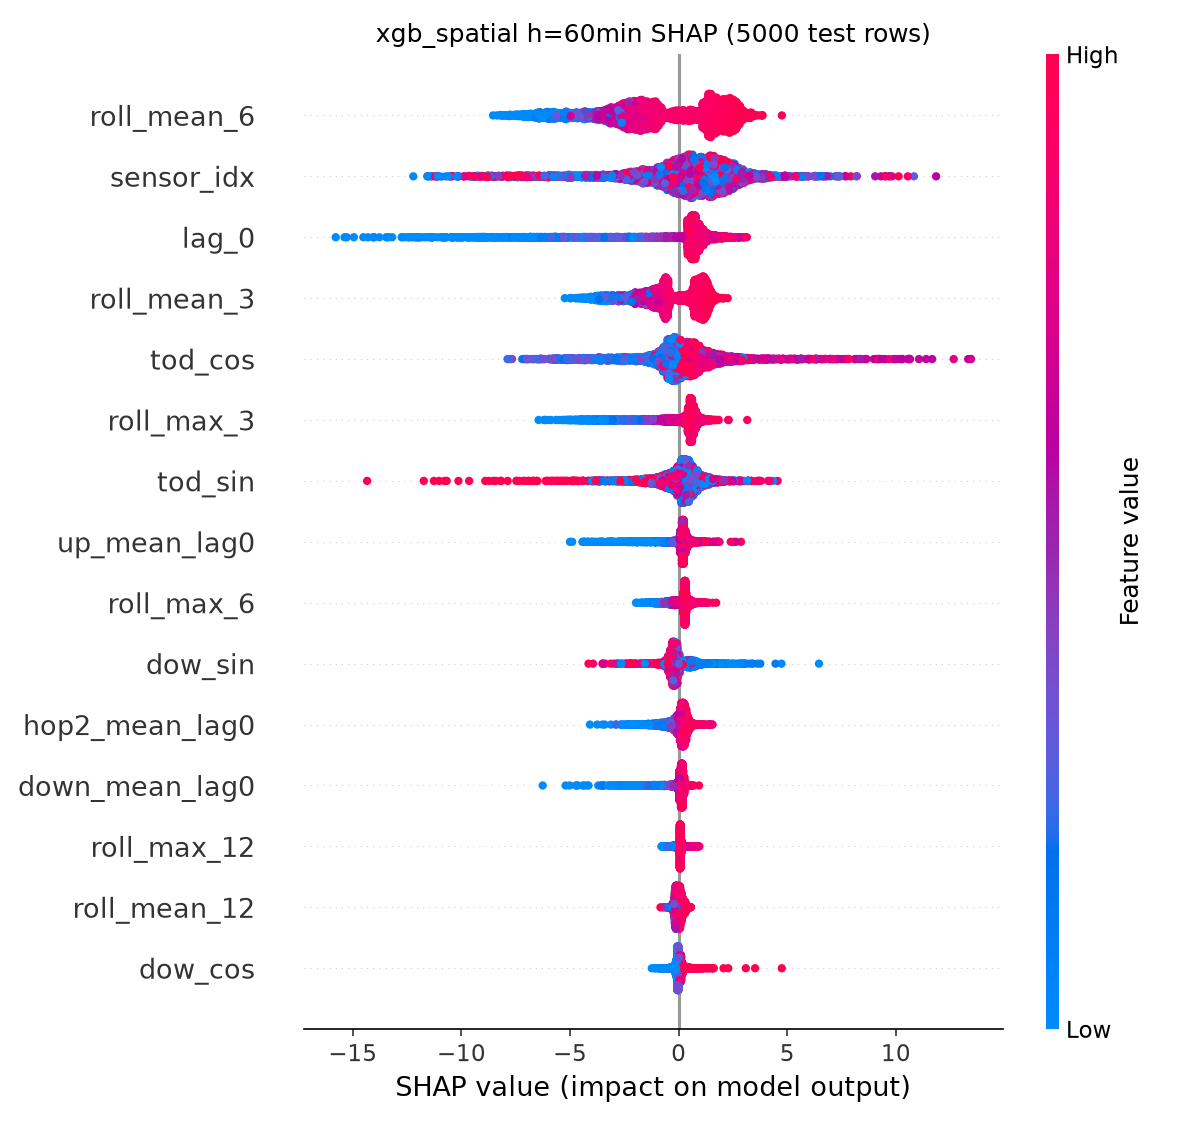
\includegraphics[width=0.9\columnwidth]{shap_xgb_spatial_h12.png}
\caption{TreeSHAP summary for XGB-spatial at 60 minutes (5,000 test rows).}\label{fig:shap}
\end{figure}

\subsection{Do hand-made neighbour features help?}
Fig.~\ref{fig:gap} shows MAE(pooled)$-$MAE(spatial) by horizon and slice.
At 15 minutes the spatial features reduce MAE by \gapAllFifteen{} mph overall (95\% CI \gapAllFifteenLo--\gapAllFifteenHi), by \gapPeakFifteen{} mph at peak versus \gapOffpeakFifteen{} off-peak, and by \gapCongestedFifteen{} mph in congestion; at 60 minutes the gains are \gapAllSixty{} (all), \gapPeakSixty{} (peak), \gapOffpeakSixty{} (off-peak) and \gapCongestedSixty{} (congested) mph.
The benefit concentrates in peaks and congestion, as the propagation hypothesis predicts, but it does not grow with horizon.
\begin{figure}[t]\centering
\includegraphics[width=\columnwidth]{gap_analysis.pdf}
\caption{Gain from neighbour features with paired block-bootstrap 95\% intervals (positive: spatial features help).}\label{fig:gap}
\end{figure}

\subsection{Graph versus no graph}
STGAT beats persistence at every horizon (\maeStgatFifteen{}/\maeStgatThirty{}/\maeStgatSixty{} versus \maePersistenceFifteen{}/\maePersistenceThirty{}/\maePersistenceSixty{} mph).
It ties the no-graph GRU at 15 minutes (\maeStgatFifteen{} vs.\ \maeGruNographFifteen{}), is slightly ahead at 30 (\maeStgatThirty{} vs.\ \maeGruNographThirty{}, not significant) and clearly ahead at 60 (\maeStgatSixty{} vs.\ \maeGruNographSixty{}, significant).
Against pooled XGBoost it is slightly worse at 15 minutes (\maeXgbGlobalFifteen{}) and better at 60 (\maeXgbGlobalSixty{}), while per-segment XGBoost stays very close (\maeXgbPerSegmentSixty{}).
The graph therefore helps where the shockwave story says it should, at long range, but modestly.

\subsection{Hybrids}
Every hybrid beats pooled XGBoost at all three horizons (Table~\ref{tab:sig}).
The residual hybrid is best at 15 and 30 minutes and the gate at 60 minutes (\maeHybridGatingSixty{} mph versus \maeStgatSixty{} for STGAT).
The residual hybrid's gain over pooled XGBoost grows with horizon (\gainXgbGlobalAllFifteen{}, \gainXgbGlobalAllThirty{}, \gainXgbGlobalAllSixty{} mph) and is largest in congestion at 60 minutes (\gainXgbGlobalCongestedSixty{} mph; \gainXgbGlobalPeakSixty{} at peak; \gainXgbGlobalFreeflowSixty{} in free flow, where it slightly hurts).
Over STGAT its gain shrinks with horizon (\gainStgatAllFifteen{}, \gainStgatAllThirty{}, \gainStgatAllSixty{} mph).
The learned gate puts more weight on STGAT at peaks than off-peak (at 60 minutes \gatePeakSixty{} versus \gateOffpeakSixty{}; Fig.~\ref{fig:gate}), as hypothesised.
\begin{figure}[t]\centering
\includegraphics[width=0.85\columnwidth]{gate_weights.pdf}
\caption{Learned gate weight on STGAT by horizon, peak versus off-peak.}\label{fig:gate}
\end{figure}
\begin{table}[t]
\centering
\caption{Diebold-Mariano statistics (negative: first model better; * p<0.05).}\label{tab:sig}
\footnotesize\resizebox{\ifdim\width>\columnwidth\columnwidth\else\width\fi}{!}{%
\begin{tabular}{lrrr}
\toprule
pair & DM@15 & DM@30 & DM@60 \\
\midrule
hybrid average vs stgat & -25.5* & -6.0* & -3.1* \\
hybrid average vs xgb global & -10.9* & -11.8* & -10.9* \\
hybrid gating vs stgat & -25.2* & -13.0* & -11.3* \\
hybrid gating vs xgb global & -12.6* & -10.6* & -9.9* \\
hybrid residual vs hybrid average & -7.2* & -5.2* & 1.1 \\
hybrid residual vs stgat & -21.3* & -9.4* & -1.3 \\
hybrid residual vs xgb global & -12.3* & -10.6* & -9.2* \\
stgat vs gru nograph & 0.4 & -6.2 & -6.8* \\
stgat vs xgb global & 4.1* & -4.7* & -5.5* \\
stgat vs xgb per segment & 6.5* & 0.3 & -0.7 \\
stgat vs xgb spatial & 17.7* & 2.4 & -3.7* \\
xgb global vs persistence & -50.4* & -34.8* & -23.0* \\
xgb global vs xgb per segment & 3.8* & 5.3* & 6.3* \\
xgb spatial vs xgb global & -14.4* & -11.5* & -6.9* \\
xgb spatial vs xgb per segment & -6.3* & -1.7 & 3.0* \\
\bottomrule
\end{tabular}}
\end{table}

\begin{figure}[t]\centering
\includegraphics[width=\columnwidth]{peak_offpeak_bars.pdf}
\caption{Error by slice at 15, 30 and 60 minutes.}\label{fig:peak}
\end{figure}

\section{Ablations}
Each ablation changes one setting from the STGAT default and was run with one seed and a reduced epoch budget (the default was re-run with the same budget as reference).
\begin{table}[t]
\centering
\caption{Ablations (1 seed, 12 epochs): MAE (mph) and change vs. default.}\label{tab:abl}
\footnotesize\resizebox{\columnwidth}{!}{%
\begin{tabular}{lrrrrrr}
\toprule
setting & MAE@15 & MAE@30 & MAE@60 & d@15 & d@30 & d@60 \\
\midrule
A0 default & 2.98 & 3.41 & 3.95 & 0.00 & 0.00 & 0.00 \\
A1 identity & 2.95 & 3.37 & 3.82 & -0.03 & -0.03 & -0.14 \\
A2 random & 3.03 & 3.48 & 4.04 & 0.04 & 0.07 & 0.09 \\
A3 backward & 2.99 & 3.42 & 3.96 & 0.01 & 0.01 & 0.00 \\
A3 forward & 3.00 & 3.42 & 3.94 & 0.01 & 0.01 & -0.01 \\
A4 gatv2 & 2.95 & 3.38 & 3.93 & -0.03 & -0.03 & -0.02 \\
A4 mean & 2.96 & 3.38 & 3.89 & -0.03 & -0.02 & -0.06 \\
A5 heads1 & 2.97 & 3.39 & 3.90 & -0.02 & -0.02 & -0.06 \\
A5 heads2 & 2.96 & 3.38 & 3.92 & -0.02 & -0.03 & -0.04 \\
A5 heads8 & 2.97 & 3.40 & 3.95 & -0.01 & -0.00 & -0.01 \\
A6 layers1 & 2.99 & 3.44 & 4.02 & 0.01 & 0.03 & 0.07 \\
A6 layers3 & 2.98 & 3.41 & 3.96 & -0.01 & 0.00 & 0.01 \\
A7 no node emb & 3.13 & 3.73 & 4.58 & 0.15 & 0.32 & 0.63 \\
A8 no time & 3.08 & 3.69 & 4.64 & 0.09 & 0.28 & 0.69 \\
A9 zero mask & 3.00 & 3.42 & 3.96 & 0.02 & 0.02 & 0.01 \\
A10 no dropout & 2.95 & 3.37 & 3.87 & -0.04 & -0.04 & -0.09 \\
A10 no wd & 2.93 & 3.31 & 3.73 & -0.06 & -0.10 & -0.22 \\
A11 H24 & 2.98 & 3.40 & 3.89 & -0.01 & -0.01 & -0.06 \\
A11 H6 & 2.98 & 3.40 & 3.93 & -0.01 & -0.01 & -0.02 \\
A12 edge bias & 2.95 & 3.37 & 3.90 & -0.03 & -0.04 & -0.06 \\
\bottomrule
\end{tabular}}
\end{table}

Under this budget the default is \emph{not} the best configuration, and the ablations do not demonstrate a benefit of the graph: the identity graph (A1, no neighbours) gives \ablAOneIdentityFifteen/\ablAOneIdentityThirty/\ablAOneIdentitySixty{} mph versus \ablAZeroDefaultFifteen/\ablAZeroDefaultThirty/\ablAZeroDefaultSixty{} for the default at 15/30/60 minutes.
A random graph with the same number of edges (A2) is worse than both (\ablATwoRandomSixty{} mph at 60 minutes), so wrong edges hurt while correct edges are about neutral at this budget.
The only large effects are removing the node embedding (A7) and the calendar features (A8), which hurt most at 60 minutes (\ablASevenNoNodeEmbSixty{} and \ablAEightNoTimeSixty{} mph).
Edge direction, attention type, heads, layers, imputation, history length and the edge bias change MAE by at most a few hundredths of a mph at 15 and 30 minutes, comparable to the seed-to-seed spread of the full runs (std \maeStgatFifteenStd{}--\maeStgatSixtyStd{} mph), so no ranking among them should be read from a single seed.
Removing dropout or weight decay helped slightly: with 12 epochs the model is under-trained rather than over-fitted.
The three-seed comparison with the GRU is the stronger evidence for a graph benefit at 60 minutes.

\section{Interpretability and Maps}
Fig.~\ref{fig:err} shows where STGAT improves on pooled XGBoost at 60 minutes during peaks (blue: STGAT better); gains cluster along specific freeway segments while a few sensors are slightly worse.
In the corridor space-time diagram (Fig.~\ref{fig:st}) neither model anticipates the abrupt breakdown near 10:00, which illustrates the difficulty of forecasting onset.
Attention is a probe, not causal evidence: averaged over test weekdays, the shares of attention on downstream-only and upstream-only neighbours are the same at the AM peak and at night (\attAmPeakDownstreamOnly\% and \attAmPeakUpstreamOnly\% versus \attNightDownstreamOnly\% and \attNightUpstreamOnly\%), so we find no peak-specific shift.
\begin{figure}[t]\centering
\includegraphics[width=\columnwidth]{error_diff_h12_peak.pdf}
\caption{Per-sensor MAE(XGB-global)$-$MAE(STGAT) at 60 min, peak hours.}\label{fig:err}
\end{figure}
\begin{figure*}[t]\centering
\includegraphics[width=0.85\textwidth]{space_time.pdf}
\caption{Corridor space-time diagram on one test day: truth and 30-minute forecasts (placed at their target time).}\label{fig:st}
\end{figure*}

\section{Simulated Ramp Metering}
\textbf{This is an offline simulation on a synthetic network. It demonstrates how forecasts could inform a control policy. No live or real-world traffic control is performed or claimed.}
METR-LA sensors are on freeways without signals, so the realistic analogue is on-ramp metering.
We simulate a 12-cell corridor with a Cell Transmission Model \cite{daganzo1994ctm} (triangular fundamental diagram, a bottleneck, three on-ramps, a 12\% capacity drop in congested cells) and compare no control, a fixed-time rate tuned on a validation day, ALINEA \cite{papageorgiou1991alinea}, a literal forecast-speed variant, and a look-ahead variant that rolls the simulator 15 minutes forward using the forecast congestion index; oracle versions use true future speeds.
Demand is synthetic, shaped by the observed congestion index (METR-LA has no flow); results are means over five test weekdays.
ALINEA reduces congested cell-minutes from \ctlNoControlCongestion{} to \ctlAlineaCongestion{} but total time spent is unchanged (\ctlNoControlTts{} versus \ctlAlineaTts{} veh$\cdot$h) because delay moves to the ramps (maximum queue \ctlAlineaMax{} veh).
The look-ahead variant behaves like ALINEA (\ctlLookaheadAlineaCongestion{} cell-minutes, \ctlLookaheadAlineaTts{} veh$\cdot$h); the literal forecast-speed variant over-meters (\ctlPredictiveAlineaTts{} veh$\cdot$h; oracle \ctlOraclePredictiveAlineaTts{}), partly because real-data forecasts do not respond to the simulator's own state.
Forecasts therefore gave no measurable benefit in this simulation (Fig.~\ref{fig:ctl}).
\begin{figure}[t]\centering
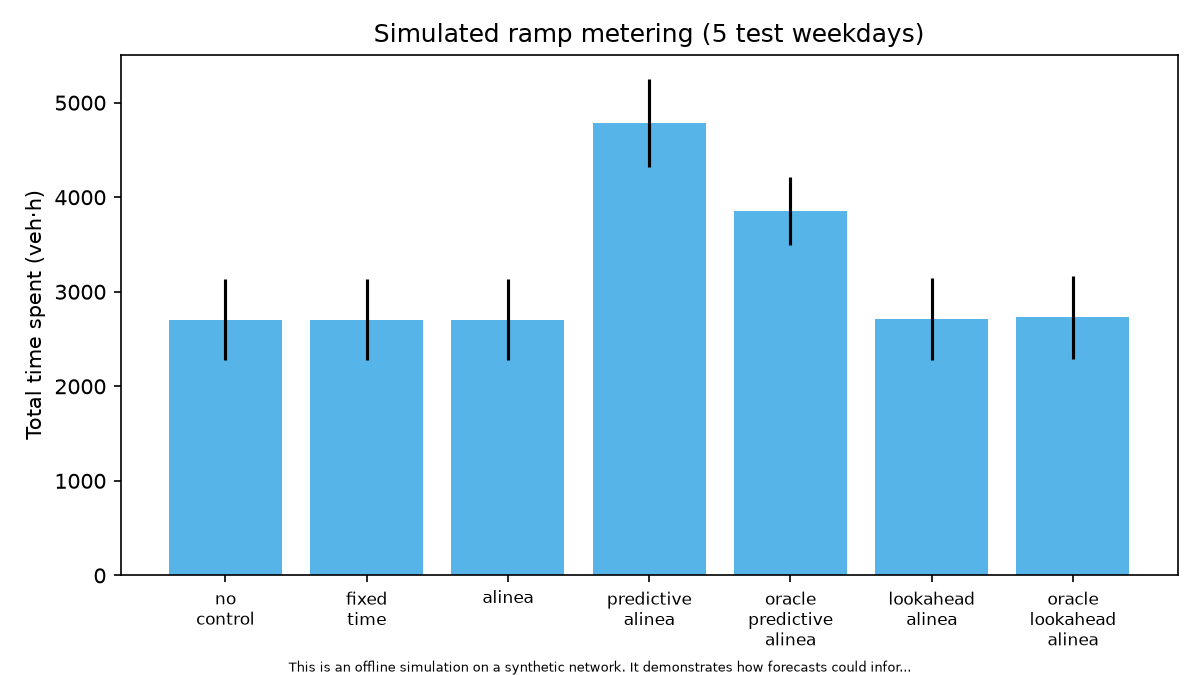
\includegraphics[width=0.9\columnwidth]{tts_by_policy.png}
\caption{Total time spent by policy in the offline simulation.}\label{fig:ctl}
\end{figure}

\section{Discussion, Limitations and Ethics}
Taken together, the evidence supports a measured version of the hypothesis: neighbour information helps most in congestion and peaks, and a learned graph model's edge appears at long range, but the effects are modest and well-tuned per-segment trees remain hard to beat; the best results come from combining them with the graph model.
Results that did not match the hypothesis are reported as found: spatial features do not help more at longer horizons; STGAT ties the GRU at 15 minutes; the ablations do not show the road graph beating a no-neighbour graph; attention does not shift between peak and night; forecasts did not help the simulated controller.
Limitations: one city and season; speed-only data; a fixed distance-based graph; reduced tuning and training budgets (including a tree cap that was always reached) and no tuning of the deep models; STGAT simplified for compute; ablations on one seed; the literature (DCRNN) protocol was not reproduced, so numbers are not directly comparable with published tables; the test period has more outages than training; MAPE is unstable at low speeds; the control study is synthetic and open loop.
The data are aggregate loop-detector speeds, so privacy risk is low; the main ethical risk is over-claiming real-world control benefits, which we avoid.
Much of the code and documentation was produced with an AI coding assistant, which we disclose.

\section{Conclusion}
Graph structure helps most at long horizons and in congestion, but modestly, and a leakage-safe combination of tuned trees and a graph attention network gives the best forecasts here: \maeHybridResidualFifteen{}, \maeHybridResidualThirty{} and \maeHybridGatingSixty{} mph at 15, 30 and 60 minutes, versus \maePersistenceFifteen{}, \maePersistenceThirty{} and \maePersistenceSixty{} for persistence.
Future work: full-budget training and tuning, learned adjacency, more seeds for ablations, flow and occupancy data (PeMS), and closed-loop control.

\bibliographystyle{IEEEtran}
\bibliography{../refs}
\end{document}
